\documentclass[conference]{../IEEEtran}

\usepackage{graphicx}
\usepackage{amsmath}
\usepackage{algorithm}
\usepackage{subfigure}
\usepackage{algpseudocode}
\usepackage{multirow}
\usepackage{pdfsync}
\usepackage{siunitx}

\newcommand{\CS}{C\nolinebreak\hspace{-.05em}\raisebox{.6ex}{\tiny\bf \#}}

\begin{document}

\title{Lab 1: Introduction to the Jaguar Lite Robot}
\author{Yukun Lin and Jennifer Zheng}

\maketitle

\begin{abstract}
This report presents proportional feedback control used to navigate the Jaguar Lite system
by Dr. Robot to a distance of \SI{1}{\meter} from a wall. A proportional gain constant
$k_{p}$ was chosen to control the robot wheel speed. Results showed a low $k_{p}$, such as
0.1, produced the desired results with minimal overshoot. When the robot reached a
steady-state value, an error on the order of \SI{0.07}{\meter} was observed due to
deadbanding.
\end{abstract}

\section{Introduction}
This paper presents a closed loop control for the Jaguar Lite robot by Dr. Robot Inc. The
robot must be able to position itself at a set distance given an initial position that may
be either farther or closer than the desired position. The use of a feedback loop allows
the robot to correct its position based on the error of its current position. A
proportional feedback control is used to achieve this goal.

\section{Problem Definition}
The goal of this lab is to design a controller that positions the robot
\SI{1}{\meter} from the wall when placed somewhere
between \SI{0.5}{\meter} and \SI{3}{\meter} from the wall. A laser range finder is
used to find the robot's position from the wall.

\section{Control Design}
%
\begin{figure}[h]
  \centering
  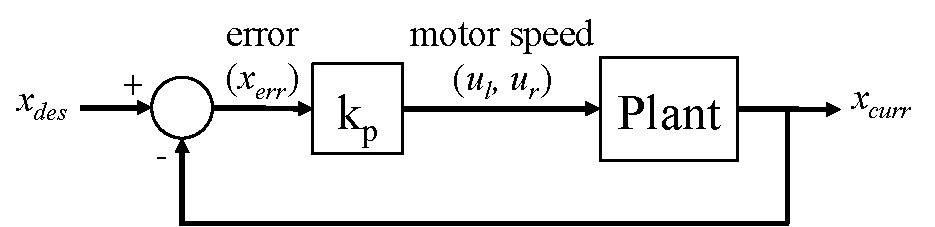
\includegraphics[width = 8cm]{figures/ControlDiagram}
  \caption{Proportional feedback control flow chart for the robot.}
  \label{fig:control}
\end{figure}
%
A proportional feedback controller was implemented in C\# to drive the robot to a desired
distance of $x_{des} =\SI{1}{\meter}$ from a wall. The distance to the wall
$x_{curr}$ is measured by the robot's laser range scanner. A proportional controller
is used to set the left and right motor speed denoted by $u_l$ and $u_r$ respectively. The
proportionality constant use is denoted by $k_p$. The flow diagram of the controller is
shown in Fig.~\ref{fig:control}, and the pseudo-code of its implementation is shown in
Alg.~\ref{alg:pc}.
%
\begin{algorithm}[b]
  \caption{Proportional Feedback Control}
  \begin{algorithmic}[1]
    \State $k_p \gets 0.1$
    \State $x_{des} \gets 1000$

    \medskip
    \While{True}
    \State $x_{err} \gets x_{des}-x_{curr}$
    \medskip
    \State $u_l \gets x_{err} * k_{p}$
    \State $u_r \gets x_{err} * k_{p}$
    \EndWhile{}

    \end{algorithmic}
  \label{alg:pc}
\end{algorithm}

The left and right wheels moved at the same speeds because the robot is assumed to start
at a position directly facing the wall, negating the need for rotation. The controller is
put in an infinite loop to drive the robot towards $x_{des}$.

\addtolength{\textheight}{-14cm}

\section{Results}

The controller was tested by placing the robot in front of a wall, on a carpeted surface.
An initial $k_p$ value of 0.4 was chosen to test the controller. The results are shown in
Fig.~\ref{fig:unstable}. Instability in the controller was observed due to the $k_p$ value
set too high relative to the update rate of the laser range finder (observed at
\SI{5}{\Hz}).
%
\begin{figure}[h]
  \centering
  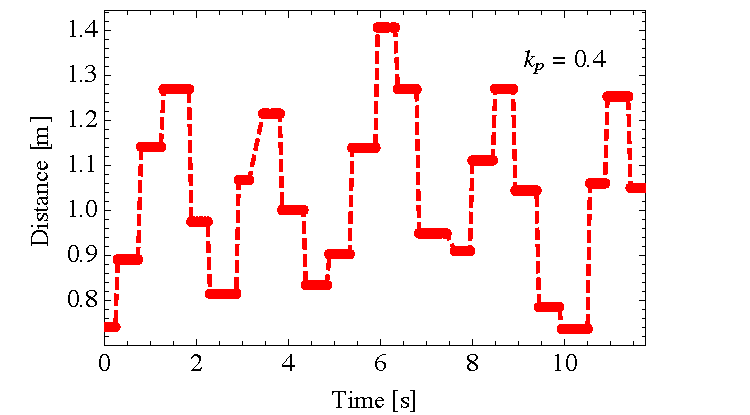
\includegraphics[width = 8cm]{figures/unstable}
  \caption{Distance of robot to wall as a function of time.
           The controller exhibits instability.}
   \label{fig:unstable}
\end{figure}
%
The $k_p$ value was then decreased to 0.15 and the results are shown in
Fig.~\ref{fig:semi_stable}. Even though the controller is now able to drive the robot
towards $x_{des}$, overshooting is observed to 1 m with minimal overshoot.
\begin{figure}[h]
  \centering
  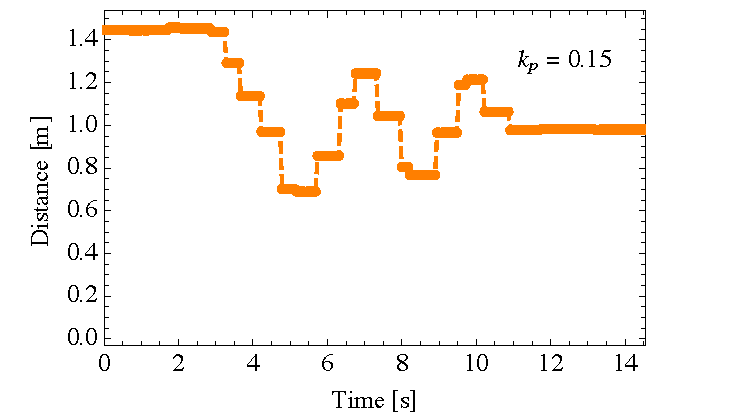
\includegraphics[width = 8cm]{figures/semi_stable}
  \caption{Distance of robot to wall as a function of time.
           The controller now exhibits overshoot.}
   \label{fig:semi_stable}
\end{figure}

\begin{figure*}[t]
  \centering
  \subfigure[]{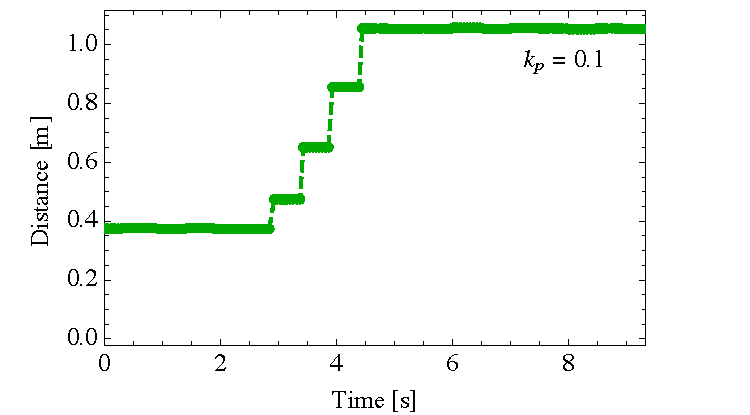
\includegraphics[width=8cm]{figures/stable_close}
  \label{fig:stable_close}}
  \subfigure[]{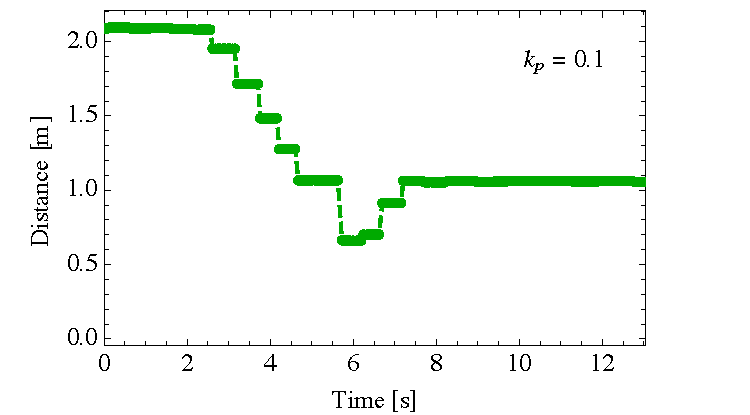
\includegraphics[width=8cm]{figures/stable_far}
  \label{fig:stable_far}}
  \caption{Distance of robot to wall as a function of time.  In (a) the robot started at a
    distance closer than \SI{1}{\meter} to the wall and in (b) it started farther than
    \SI{1}{\meter}. The controller reaches a steady-state value with no or minimal
  overshoot in both cases.}
  \label{fig:stable_controller}
\end{figure*}

The $k_p$ value was decreased to 0.1 to prevent overshooting. Fig.~\ref{fig:stable_close}
and Fig.~\ref{fig:stable_far} show the robot starting at a distance below and above
$x_{des}$. The robot is able to reach a steady-state value close to $x_{des}$.

The three cases described by
Fig.~\ref{fig:semi_stable},~\ref{fig:stable_close},~\ref{fig:stable_far} show the robot
reach a steady-state value that is, at most, \SI{0.07}{\meter} from \SI{1}{\meter}. This is due to
deadbanding. A deadband is an area where a physical system cannot perform what the control
signal specifies. As the robot gets close to the desired position, the motor speed is set
too low for the robot to physically move.

\section{Conclusion}
This report presents a proportional feedback control implemented on the Jaguar Lite system
by Dr. Robot to navigate the robot to a distance of \SI{1}{\meter} from the wall. A
proportional gain constant of $k_{p} = 0.1$ was found to be able to drive the robot closed
to the desired distance. Due to deadbanding, an error of \SI{0.07}{\meter} was
observed when the robot came to a halt.

\end{document}
